\documentclass[]{book}

%These tell TeX which packages to use.
\usepackage{array,epsfig}
\usepackage{amsmath}
\usepackage{amsfonts}
\usepackage{amssymb}
\usepackage{amsxtra}
\usepackage{amsthm}
\usepackage{mathrsfs}
\usepackage{color}
\usepackage{enumitem}
%Here I define some theorem styles and shortcut commands for symbols I use often
\theoremstyle{definition}
\newtheorem{defn}{Definition}
\newtheorem{thm}{Theorem}
\newtheorem{cor}{Corollary}
\newtheorem*{rmk}{Remark}
\newtheorem{lem}{Lemma}
\newtheorem*{joke}{Joke}
\newtheorem{ex}{Example}
\newtheorem*{soln}{Solution}
\newtheorem{prop}{Proposition}

\newcommand{\lra}{\longrightarrow}
\newcommand{\ra}{\rightarrow}
\newcommand{\surj}{\twoheadrightarrow}
\newcommand{\graph}{\mathrm{graph}}
\newcommand{\bb}[1]{\mathbb{#1}}
\newcommand{\Z}{\bb{Z}}
\newcommand{\Q}{\bb{Q}}
\newcommand{\R}{\bb{R}}
\newcommand{\C}{\bb{C}}
\newcommand{\N}{\bb{N}}
\newcommand{\M}{\mathbf{M}}
\newcommand{\m}{\mathbf{m}}
\newcommand{\MM}{\mathscr{M}}
\newcommand{\HH}{\mathscr{H}}
\newcommand{\Om}{\Omega}
\newcommand{\Ho}{\in\HH(\Om)}
\newcommand{\bd}{\partial}
\newcommand{\del}{\partial}
\newcommand{\bardel}{\overline\partial}
\newcommand{\textdf}[1]{\textbf{\textsf{#1}}\index{#1}}
\newcommand{\img}{\mathrm{img}}
\newcommand{\ip}[2]{\left\langle{#1},{#2}\right\rangle}
\newcommand{\inter}[1]{\mathrm{int}{#1}}
\newcommand{\exter}[1]{\mathrm{ext}{#1}}
\newcommand{\cl}[1]{\mathrm{cl}{#1}}
\newcommand{\ds}{\displaystyle}
\newcommand{\vol}{\mathrm{vol}}
\newcommand{\cnt}{\mathrm{ct}}
\newcommand{\osc}{\mathrm{osc}}
\newcommand{\LL}{\mathbf{L}}
\newcommand{\UU}{\mathbf{U}}
\newcommand{\support}{\mathrm{support}}
\newcommand{\AND}{\;\wedge\;}
\newcommand{\OR}{\;\vee\;}
\newcommand{\Oset}{\varnothing}
\newcommand{\st}{\ni}
\newcommand{\wh}{\widehat}

%Pagination stuff.
\setlength{\topmargin}{-.3 in}
\setlength{\oddsidemargin}{0in}
\setlength{\evensidemargin}{0in}
\setlength{\textheight}{9.in}
\setlength{\textwidth}{6.5in}
\pagestyle{empty}


\begin{document}

\begin{center}
{\Large Data 227 - Autumn 2023 \hspace{0.5cm} HW 3}\\
\textbf{Data Visualization and Communication - Trimble}\\ %You should put your name here
Due: Friday October 20, 2023  11:59pm   
\end{center}

\vspace{0.2 cm}

\subsection*{Fireball data}

\begin{enumerate} 
\item\label{boldie}

The Center for Near Earth Object Studies has collected a database of large, bright objects that have impacted the Earth and were detected by the flashes they made, day or night, in the atmosphere (Fireball and Bolide Data, Center for Near Earth Object Studies). As of Oct 13, 2023 the list has 964 events.

\texttt{https://cneos.jpl.nasa.gov/fireballs/}

This question asks you to create effective visualizations of the distribution of variables related to these fireballs.

\begin{enumerate} [label=\alph*]
\item For all of the columns in the database, consider the nature of each variable–should we expect the variables to be numerical (discrete or continuous)? Categorical (nominal or ordinal)? Write down what you expect without viewing the storage types of the data. (1 pt)
\item  Now, read in the data.  If any of the storage types need to be converted, convert them.  Convert the date and time to a time data type. (1 point)
\item  Is there anything unusual about the distribution of date and times of fireballs in the dataset? (1 pt)
\item  For visualizing distributions, histograms or cumulative distribution plots are suitable. Visualize the distribution of longitudes using a histogram, and describe the center, shape, and spread of the distribution. Indicate the presence of any outliers. Is this distribution consistent with what you might expect? (1 pts)
\item  Visualize the distribution of the latitudes.  Is this distribution consistent with what you might expect? (1 pts)
\item  Plot a histogram of Total Impact Energies, and describe the center, shape, and spread of the distribution. Indicate the presence of any outliers.  Do some of the outliers have their own wikipedia pages?  Is this distribution consistent with what you might expect? (1 pts)
\item  For right-skewed graphs, a log-scale is often appropriate for visualizing differences in the data. Plot the distribution of transformed Total Impact Energies using a histogram, and describe the center, shape, and spread of the distribution. Indicate the presence of any outliers. Do your findings change from Part f? (2 pts)
\item Count the number of fireballs in each degree of longitude.  Make a plot that compares the histogram-of-the-histogram (number of degrees of longitude with 0, 1, 2, etc.  events)  with the Poisson distribution with the same number of average events.    This will be a Poisson distribution with a mean of 964 / 180.  Comment on their agreement / disagreement. (2pts)

\end{enumerate}

%\begin{figure}
%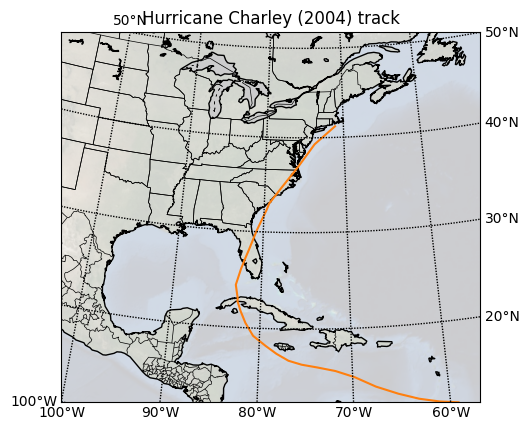
\includegraphics[width=12cm]{Charley.png}
%\caption{Sample code to produce this map is provided}
%\end{figure}

\subsection*{Birth data }
\item\label{births}

For this problem, you will create a static visualization from the CDC birth database.  Data for births and infant deaths is available from the CDC Vital Statistics Online Portal 

\texttt{https://www.cdc.gov/nchs/data\_access/vitalstatsonline.htm }.

The CDC, for fifty years, has been compiling data about each birth in the United States, making most of the data from these standard forms available. This data consists of about 50 fields, almost all of which are categorical data referring to geography, presence of absence of risk factors, method of delivery, duration of gestation, age of parents, date of birth, etc. This will require some amount of effort to wrangle.  There are myriad relationships in this dataset, and hundreds of papers have been written leveraging the birth census for making inferences about maternal and infant health.

There are 2-4 million births and about 20,000 infant deaths per year.  Different years have different sets of fields. Examine the data, find a fact that is contained within the data, and design a visualization that communicates that fact.(6pts)

Include a figure caption and just one paragraph discussing your findings and the graphical design. (1pt) Attach any code you used to produce the visualization. The figure caption should describe the origin of the dataset.(1pt)

%#You do not have to use any specific tools to produce the visualization (you could even draw it by hand) but you need to find something interesting and display it effectively.

Please put your question 2 visualization in a PDF of its own, with its caption, separate from the code.  ( 2 points)
%\begin{soln}
%	% Put your answers here.
%\end{soln}


\end{enumerate}

\end{document}


